\documentclass[]{article}
\usepackage{graphicx}
\usepackage[svgnames]{xcolor} 
\usepackage{fancyhdr}
\usepackage{tocloft}
\usepackage[hidelinks]{hyperref}
\usepackage{enumitem}
\usepackage[many]{tcolorbox}
\usepackage{listings }
%\usepackage[a4paper, total={6in, 8in} , top = 2cm,bottom = 4cm]{geometry}
\usepackage[a4paper, total={6in, 8in}]{geometry}
\usepackage{afterpage}
\usepackage{amssymb}
\usepackage{hyperref}
\usepackage{pdflscape}
\usepackage{textcomp}
\usepackage{xecolor}
\usepackage{rotating}
\usepackage{xepersian}
\usepackage[T1]{fontenc}
\usepackage{tikz}
\usepackage[utf8]{inputenc}
\usepackage{PTSerif} 
\usepackage{seqsplit}
\usepackage{changepage}


\usepackage{listings}
\usepackage{xcolor}
\usepackage{sectsty}

\setcounter{secnumdepth}{0}
 
\definecolor{codegreen}{rgb}{0,0.6,0}
\definecolor{codegray}{rgb}{0.5,0.5,0.5}
\definecolor{codepurple}{rgb}{0.58,0,0.82}
\definecolor{backcolour}{rgb}{0.95,0.95,0.92}
\definecolor{blanchedalmond}{rgb}{1.0, 0.92, 0.8}
\definecolor{brilliantlavender}{rgb}{0.96, 0.73, 1.0}
 
\NewDocumentCommand{\codeword}{v}{
\texttt{\textcolor{blue}{#1}}
}
\lstset{language=java,keywordstyle={\bfseries \color{blue}}}

\lstdefinestyle{mystyle}{
    backgroundcolor=\color{backcolour},   
    commentstyle=\color{codegreen},
    keywordstyle=\color{magenta},
    numberstyle=\tiny\color{codegray},
    stringstyle=\color{codepurple},
    basicstyle=\ttfamily\normalsize,
    breakatwhitespace=false,         
    breaklines=true,                 
    captionpos=b,                    
    keepspaces=true,                 
    numbers=left,                    
    numbersep=5pt,                  
    showspaces=false,                
    showstringspaces=false,
    showtabs=false,                  
    tabsize=2
}

\lstset{style=mystyle}

 \settextfont[BoldFont={XB Zar bold.ttf}]{XB Zar.ttf}


\setlatintextfont[Scale=1.0,
 BoldFont={LiberationSerif-Bold.ttf}, 
 ItalicFont={LiberationSerif-Italic.ttf}]{LiberationSerif-Regular.ttf}





\newcommand{\inputsample}[1]{
    ~\\
    \textbf{ورودی نمونه}
    ~\\
    \begin{tcolorbox}[breakable,boxrule=0pt]
        \begin{latin}
            \large{
                #1
            }
        \end{latin}
    \end{tcolorbox}
}

\newcommand{\outputsample}[1]{
    ~\\
    \textbf{خروجی نمونه}

    \begin{tcolorbox}[breakable,boxrule=0pt]
        \begin{latin}
            \large{
                #1
            }
        \end{latin}
    \end{tcolorbox}
}

\newtcolorbox{mybox}[2][]{colback=red!5!white,
colframe=red!75!black,fonttitle=\bfseries,
colbacktitle=red!85!black,enhanced,
attach boxed title to top center={yshift=-2mm},
title=#2,#1}

\newenvironment{changemargin}[2]{%
\begin{list}{}{%
\setlength{\topsep}{0pt}%
\setlength{\leftmargin}{#1}%
\setlength{\rightmargin}{#2}%
\setlength{\listparindent}{\parindent}%
\setlength{\itemindent}{\parindent}%
\setlength{\parsep}{\parskip}%
}%
\item[]}{\end{list}}


\definecolor{foldercolor}{RGB}{124,166,198}
\definecolor{sectionColor}{HTML}{ff5e0e}
\definecolor{subsectionColor}{HTML}{008575}

\definecolor{listColor}{HTML}{00d3b9}

\definecolor{umlrelcolor}{HTML}{3c78d8}

\definecolor{subsubsectionColor}{HTML}{3c78d8}

\definecolor{CustomColor}{HTML}{A61C00}


\defpersianfont\authorFont[Scale=0.9]{XB Zar bold.ttf}

\defpersianfont\titr[Scale=1.5]{Lalezar-Regular.ttf}

\defpersianfont\fehrest[Scale=1.2]{Lalezar-Regular.ttf}

\defpersianfont\fehrestTitle[Scale=3.0]{Lalezar-Regular.ttf}

\defpersianfont\fehrestContent[Scale=1.2]{XB Zar bold.ttf}


\sectionfont{\color{sectionColor}}  % sets colour of sections
\subsectionfont{\color{subsectionColor}}  % sets colour of sections
\subsubsectionfont{\color{subsubsectionColor}}


\renewcommand{\labelitemii}{$\circ$}


\renewcommand{\baselinestretch}{1.1}


\renewcommand{\contentsname}{فهرست}

\renewcommand{\cfttoctitlefont}{\fehrestTitle}


\renewcommand\cftsecfont{\color{sectionColor}\fehrestContent\selectfont}
\renewcommand\cftsubsecfont{\color{subsectionColor}\fehrestContent\selectfont}
\renewcommand\cftsubsubsecfont{\color{subsubsectionColor}\fehrestContent\selectfont}
%\renewcommand{\cftsecpagefont}{\color{sectionColor}}

\setlength{\parskip}{1.2pt}

\begin{document}


%%% title pages
\begin{titlepage}
\begin{center}

\textbf{ \Huge{به نام خدا} }
        
\vspace{0.2cm}


\includegraphics[width=0.4\textwidth]{Logo/aut-fa2.png}\\
\vspace{0.2cm}
\textbf{ \Huge{\emph درس مدار‌های منطقی} }\\
\vspace{0.25cm}
\textbf{ \Large{ پروژه نهایی} }
\vspace{0.2cm}
       
 
      \large \textbf{دانشکده مهندسی کامپیوتر}\\\vspace{0.1cm}
    \large   دانشگاه صنعتی امیرکبیر\\\vspace{0.2cm}
       \large   ﻧﯿﻢ سال دوم ۰۳-۰۲ \\\vspace{0.10cm}
      \noindent\rule[1ex]{\linewidth}{1pt}
استاد:\\
    \textbf{{دکتر مرتضی صاحب‌الزمانی}}



    \vspace{0.20cm}

   مهلت ارسال و ارائه:\\
    \textbf{{17 تیر}}

    \vspace{0.10cm}
مسئول پروژه:\\
    \textbf{\authorFont{مدرسین آزمایشگاه منطقی}}
    
        \vspace{0.10cm}
طراحان پروژه:\\
    \textbf{\authorFont{ رضا آدینه پور، محمد مهدی نعمتی }}
    

\end{center}
\end{titlepage}
%%% title pages


%%% header of pages
\newpage
\pagestyle{fancy}
\fancyhf{}
\fancyfoot{}
\cfoot{\thepage}
\lhead{نیمسال ۰۳-۰۲}
\rhead{
\includegraphics[width=0.1\textwidth]{Logo/ce-fa.png}\\
دانشکده مهندسی کامپیوتر
}
\chead{پروژه مدارمنطقی}
%%% header of pages
\renewcommand{\headrulewidth}{2pt}



\tableofcontents

\newpage

 \Large \textbf{\\
}

\section*{{\titr نکات قابل توجه}}
\addcontentsline{toc}{section}{{\fehrestContent نکات قابل توجه}}
\begin{itemize}
	
\item 
ددلاین تحویل فاز اول پروژه، در روز‌های \textbf{شنبه، ۱۹} و \textbf{دوشنبه، ۲۱ خرداد}\footnote{هر گروه در زمان کلاس خودش} در کلاس آزمایشگاه است. همچنین تحویل فاز دوم پروژه، \textbf{یکشنبه ۱۷ تیر} خواهد بود.
	
\item
انجام پروژه به‌صورت گروهی‌ست و گروه‌های شما همان گروه‌های آزمایشگاه است. درصورت وجود مشکل موجه، با هماهنگی با مدرسین آزمایشگاه می‌توانید گروه خود را تغییر دهید.


\item
دانشجویان \textbf{ملزم به تحویل حضوری} هر دو فاز پروژه هستند. درصورتی که گروهی در روز تحویل حاضر نشود نمره‌ای به ایشان تعلق نخواهد گرفت.

\item
در روز تحویل حضوری مشارکت تمام اعضای تیم در پروژه بررسی خواهد‌ شد و در صورت عدم مشارکت بعضی از اعضا، نمرهٔ ایشان برای آن فاز از پروژه "صفر" لحاظ می‌گردد. مشارکت، با توجه به commit های افراد تیم در مخزن گیت‌هاب پروژه و سوالات پرسیده شده در روز تحویل و با صلاحدید مدرس مشخص می‌شود.

\item 
ساختار ماژولار کد ها حتما باید حفظ شود درصورت عدم رعایت، منفی نمره آن قسمت برای اعضای گروه ثبت خواهد شد.

\item
ددلاین فاز اول و دوم در آخرین زمان ممکن قبل از تحویل نمرات قرار داده شده است. لذا در هر دو فاز \textbf{مهلت تاخیر وجود ندارد}.

\item
در صورت کشف تقلب از هریک از تیم‌ها، برای بار اول منفی نمرهٔ آن فاز برای آن تیم ثبت می‌شود و برای بار دوم، نمرهٔ منفی کل پروژه برای تیم لحاظ خواهد‌ شد که معادل \textbf{مردود شدن} در درس است.
\end{itemize}

\newpage



 \Large \textbf{\\
}

\section*{{\titr مقدمه}}
\addcontentsline{toc}{section}{{\fehrestContent مقدمه}}


\subsection*{{\titr یعقوب\footnote{\lr{Electronic Jacob}} برقی که بود؟}}
\addcontentsline{toc}{subsection}{{\fehrestContent یعقوب برقی که بود؟}}

\textbf{هر امیرکبیری میدونه!}

که اسم جهانی یعقوب برقی\footnote{برگرفته از یعقوب آقا، دکه وسط صحن دانشگاه} مخصوص دستگاه‌های فروش خودکار است که اگر با همین نام اون رو در گوگل سرچ کنید متوجه جهانی بودن این اسم می‌شوید.


\begin{figure}[h]
	\centering
	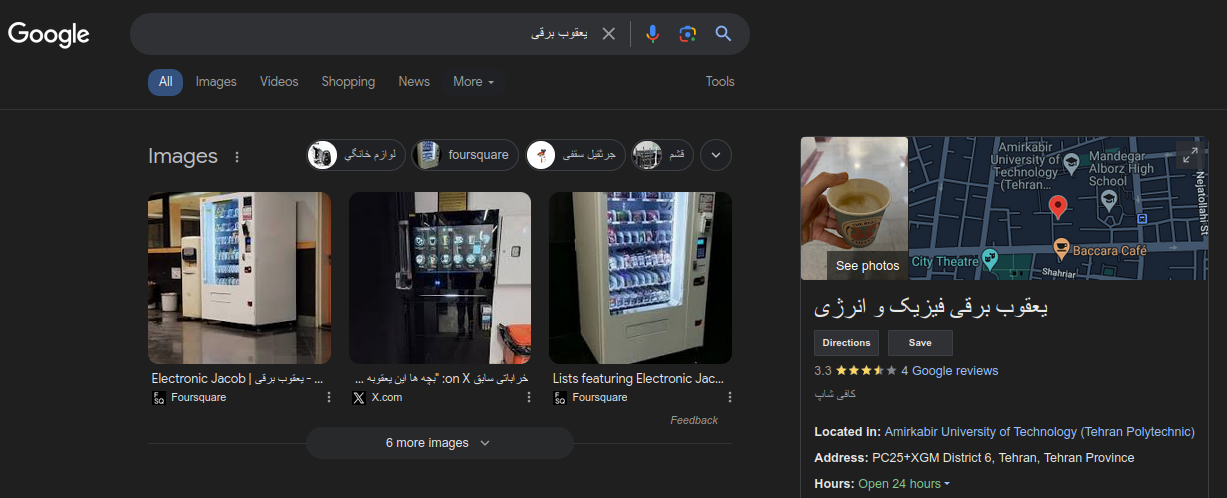
\includegraphics[width=1\textwidth]{images/img1}
	\caption{این نام جهانیست!}
	\label{این نام جهانیست!}
\end{figure}








احتمالا همگی یعقوب برقی دانشکده رو دیدین و از اون استفاده کردین.

در این پروژه قصد داریم کمی بیشتر با یعقوب برقی آشنا بشیم و بخش کوچکی از سیستم کنترلی اون رو طراحی، شبیه‌سازی و پیاده سازی کنیم.

بعد از انجام این پروژه، خرید‌های شما از یعقوب برقی، فقط یک خرید ساده نیست!




\Large \textbf{\\\\\\
}


\subsection*{{\titr اهداف پروژه}}
\addcontentsline{toc}{subsection}{{\fehrestContent اهداف پروژه}}
\begin{itemize}
	\item
	هدف این پروژه، طراحی و شبیه‌سازی سیستم کنترلی دستگاه فروش خودکار است که در فاز صفر آن صرفا \lr{FSM} های کلی پروژه طراحی و مخزن\footnote{\lr{Repository}} گیتهاب پروژه راه اندازی می‌شود. 
	
	\item 
	در فاز اول، می‌بایست \lr{FSM} های کشیده شده در فاز صفر تکمیل شوند، طوری که تمام حالات پوشش داده شود و همچنین کد طراحی انجام شده به زبان \lr{Verilog} نوشته شود و بر روی \lr{FPGA} پیاده‌سازی شود.
	\item 
	آشنایی با سیستم مدیریت نسخه \lr{Git} و کار تیمی بر روی پروژه بر بستر یک مخزن \lr{Github}، یکی دیگر از اهداف پروژه است. در این مورد توصیه می‌شود تغییرات خود را در دوره‌های کوتاه مدت \lr{commit} کنید.
\end{itemize}



 \Large \textbf{\\
}


\section*{{\titr توضیحات کلی }}
\addcontentsline{toc}{section}{{\fehrestContent توضیحات کلی}}
\label{sec:detail}

پروژه در ۲ حالت\footnote{\lr{Mode}} کاری طراحی شده است.
\begin{itemize}
	\item حالت مدیر\footnote{\lr{Admin}}
	\item حالت کاربر\footnote{\lr{User}}
\end{itemize}

بنابر این پروژه باید دارای ۳ ماژول اصلی ماژول \lr{\texttt{admin.v}}، \lr{\texttt{user.v}} و  \lr{\texttt{main.v}} باشد. زیر ماژول های هرکدام در ادامه توضیح داده خواهد شد.





\newpage
\Large \textbf{\\
}

\subsection*{{\titr حالت مدیر}} 
\addcontentsline{toc}{subsection}{{\fehrestContent حالت مدیر}}
سیستم پس از روشن شدن به‌صورت پیش‌فرض در حالت کاربر روشن می‌شود. با نگه داشتن ۵ ثانیه‌ای یکی از \lr{Push button} های موجود بر روی بُرد وارد حالت مدیر می‌شویم.

هر دستگاه پسوردی دارد که تنها مدیر دستگاه با وارد کردن آن می‌تواند وارد این حالت شود. پسورد دستگاه به صورت زیر درنظر گرفته شود:

\begin{latin}
	\texttt{Admin\_pass: 02}
\end{latin}



مقدار پسورد باید جایی در حافظه رجیستر شود و در زمان عوض کردن حالت کاری سیستم، پسورد وارد شده توسط شخص با مقدار از قبل ذخیره شده مقایسه شود.

شخص می‌تواند برای وارد کردن پسورد از \lr{Dip switch} های بُرد استفاده کند. پس از وارد شدن به حالت مدیر، مدیر می‌تواند اجناس دستگاه را مطابق با شماره خانه های یعقوب برقی دانشکده (شکل «\textcolor{blue}{\ref{یعقوب برقی دانشکده}}») شارژ کند



\begin{figure}[h]
	\centering
	
\includegraphics[width=0.4\textwidth]{images/img2.jpg}
	\caption{یعقوب برقی دانشکده}
	\label{یعقوب برقی دانشکده}
\end{figure}

\newpage
\Large \textbf{\\
}

همچنان برای انتخاب جایگاه موردنظر از \lr{Dip switch} ها استفاده کنید و برای مشخص کردن تعداد اجناس قرار داده شده در جایگاه انتخاب شده از ۲ \lr{Push button} بُرد استفاده کنید. یکی از \lr{Push button} ها بالا شمار و دیگری پایین شمار فرض شود. برای راحتی فرض‌های زیر انجام شود:

\begin{itemize}
	\item موجودی تمامی جایگاه ها در ابتدای کار صفر است
	\item هر جایگاه حداکثر ۱۰ ظرفیت دارد
	\item قیمت اجناس ردیف اول\footnote{ترتیب ردیف‌ها از بالا بیان شده} ۸۵۰۰ تومان
	\item ردیف دوم، ۶۰۰۰ تومان
	\item ردیف سوم ۴۵۰۰
	\item ردیف چهارم ۳۰۰۰ تومان
	\item و ردیف ۵ و ۶ هر کدام ۲۰۰۰ تومان
\end{itemize}

برای خروج از حالت مدیر می‌بایست شماره جایگاه‌ دستگاه را بر روی صفر قرار دهید. درصورت فراموشی مدیر برای خروج از حالت مدیر، برای حفظ امنیت، دستگاه می‌بایست به‌صورت خودکار پس از ۱ دقیقه از حالت مدیر خارج شده و به حالت کاربر برگردد.



ماژول طراحی شده در این قسمت باید به‌صورت زیر باشد:


\begin{figure}[h]
	\centering
	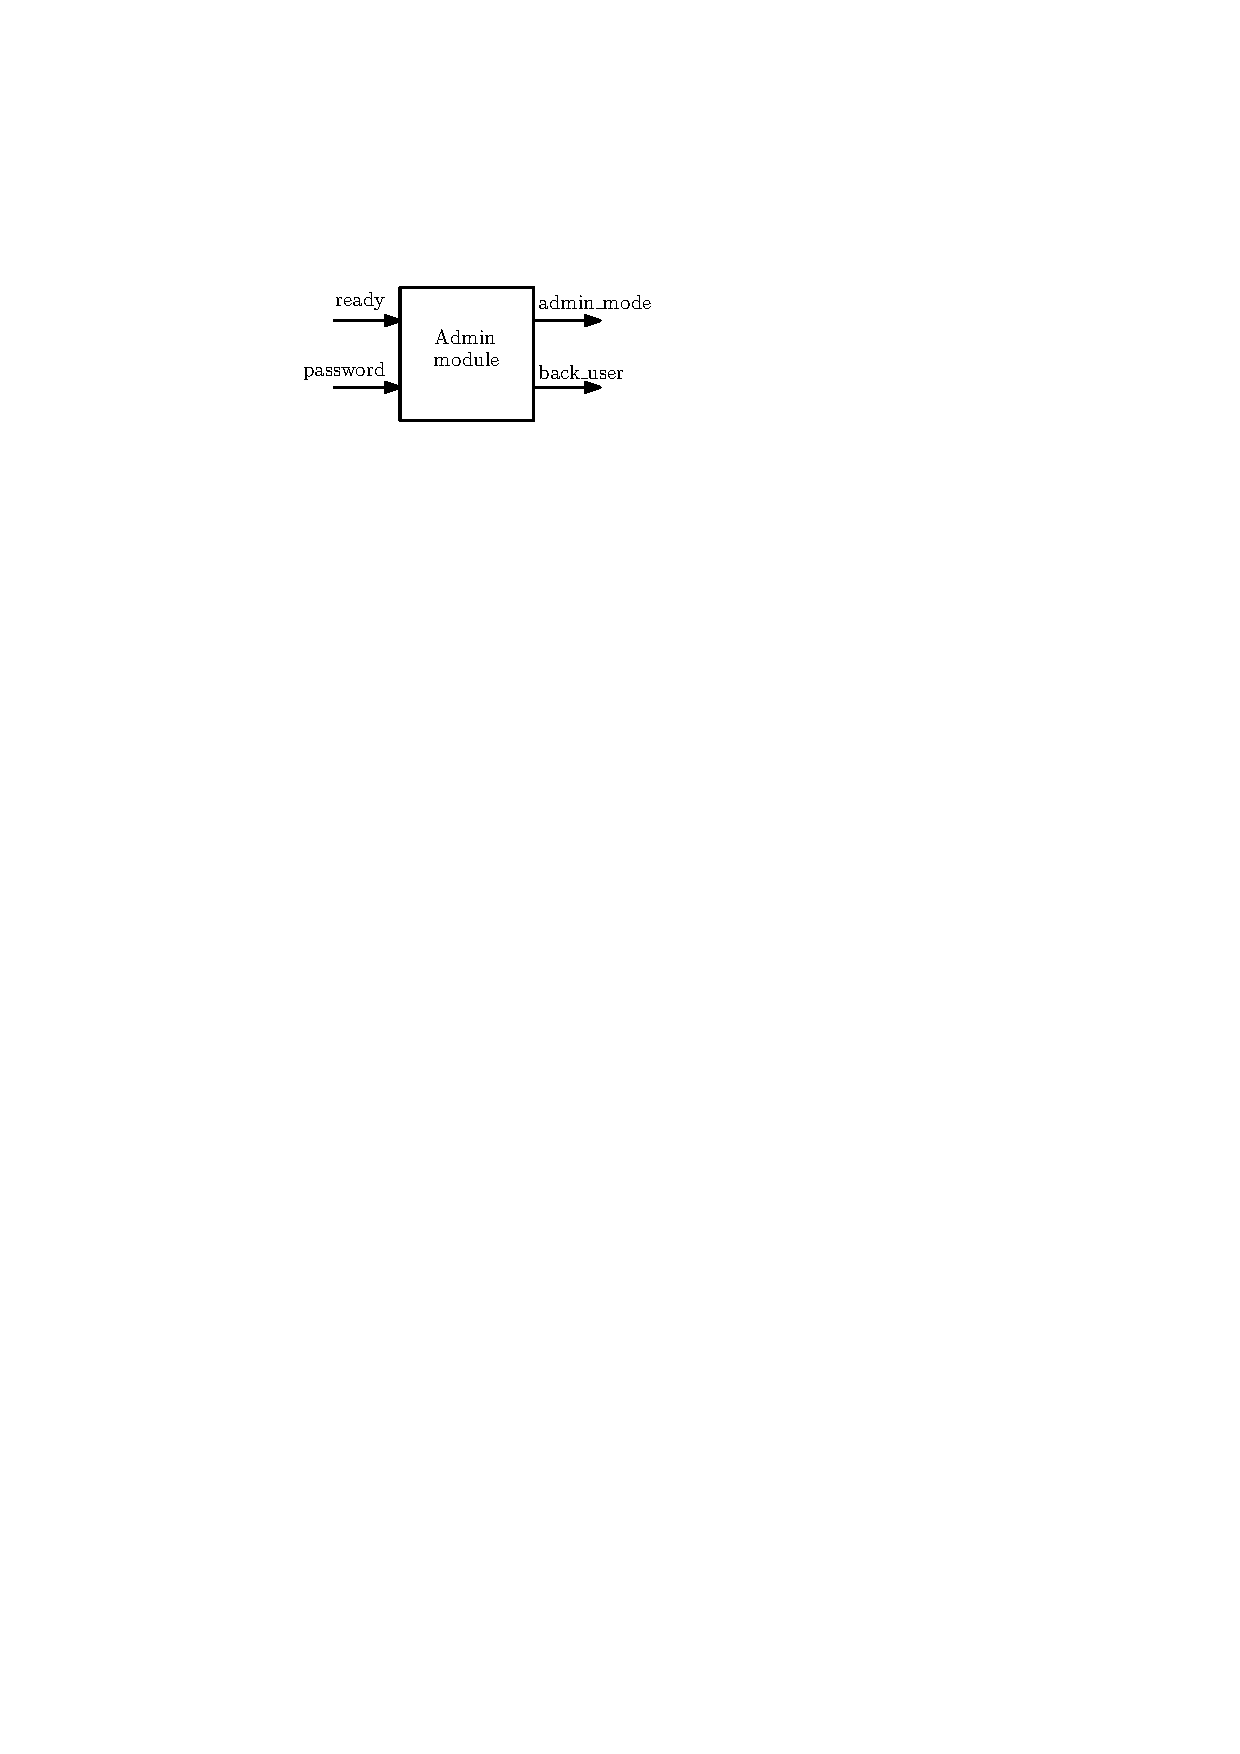
\includegraphics[width=0.5\textwidth]{images/admin.pdf}
	\caption{ماژول \texttt{admin.v}}
	\label{ماژول admin.v}
\end{figure}

 (خروجی های \lr{\texttt{admin\_mode}} و \lr{\texttt{back\_user}} حالت کاری سیستم را نشان می‌دهند که باید به دو \lr{LED} متصل شوند.)



\newpage
\Large \textbf{\\
}




\subsection*{{\titr حالت کاربر}} 
\addcontentsline{toc}{subsection}{{\fehrestContent حالت کاربر}}
در این حالت، کاربران می‌توانند شماره جنس مورد نظر خود را انتخاب کنند و درصورت موجود بودن کالا و داشتن موجودی مالی، آن را خریداری کنند. برای سادگی فرض می‌شود ۳ کاربر داریم که مقدار موجودی حساب هرکدام به‌صورت زیر است:

\begin{itemize}
	\item کاربر ۱: ۷۰۰۰ تومان
	\item کاربر ۲: ۵۰۰۰ تومان
	\item کاربر ۳: ۳۰۰۰ تومان 
\end{itemize}

انتخاب کاربر‌ها با استفاده از \lr{Dip switch} ها انجام می‌شود و فعال بودن هرکدام می‌بایست بر روی \lr{LED} ها نمایش داده شود.

پس از انتخاب کاربر، موجودی آن باید بر روی \lr{Seven segment} نمایش داده شود. کاربر پس از انتخاب کالای مورد نظر خود و تایید خرید (با استفاده از \lr{Push button}) درصورت داشتن موجودی کافی در حساب کاربر و دستگاه، خرید با موفقیت انجام می‌شود و مانده حساب آپدیت شده و نمایش داده می‌شود.

موجودی هر کالا پس از انتخاب آن توسط کاربر می‌بایست بر روی \lr{LED} ها نمایش داده شود.

درنظر گرفتن موارد زیر الزامیست:

\begin{enumerate}
	\item هرکاربر می‌تواند چندین بار خرید انجام دهد.
	\item درصورت موجود نبودن کالا می‌بایست پیغام مناسب داده شود و فرایند خرید پایان یابد
	\item درصورت نداشتن موجودی حساب، کاربر اصلا نباید وارد فرایند خرید شود
	\item پس از اتمام خرید، موقعیت جایگاه دستگاه بر روی حالت قبلی می‌ماند اما تا تایید نکردن خرید نباید فرآیند خرید آغاز شود
\end{enumerate}



ماژول طراحی شده در این قسمت باید به‌صورت زیر باشد:
\newpage
\Large \textbf{\\\\
}

\begin{figure}[h]
	\centering
	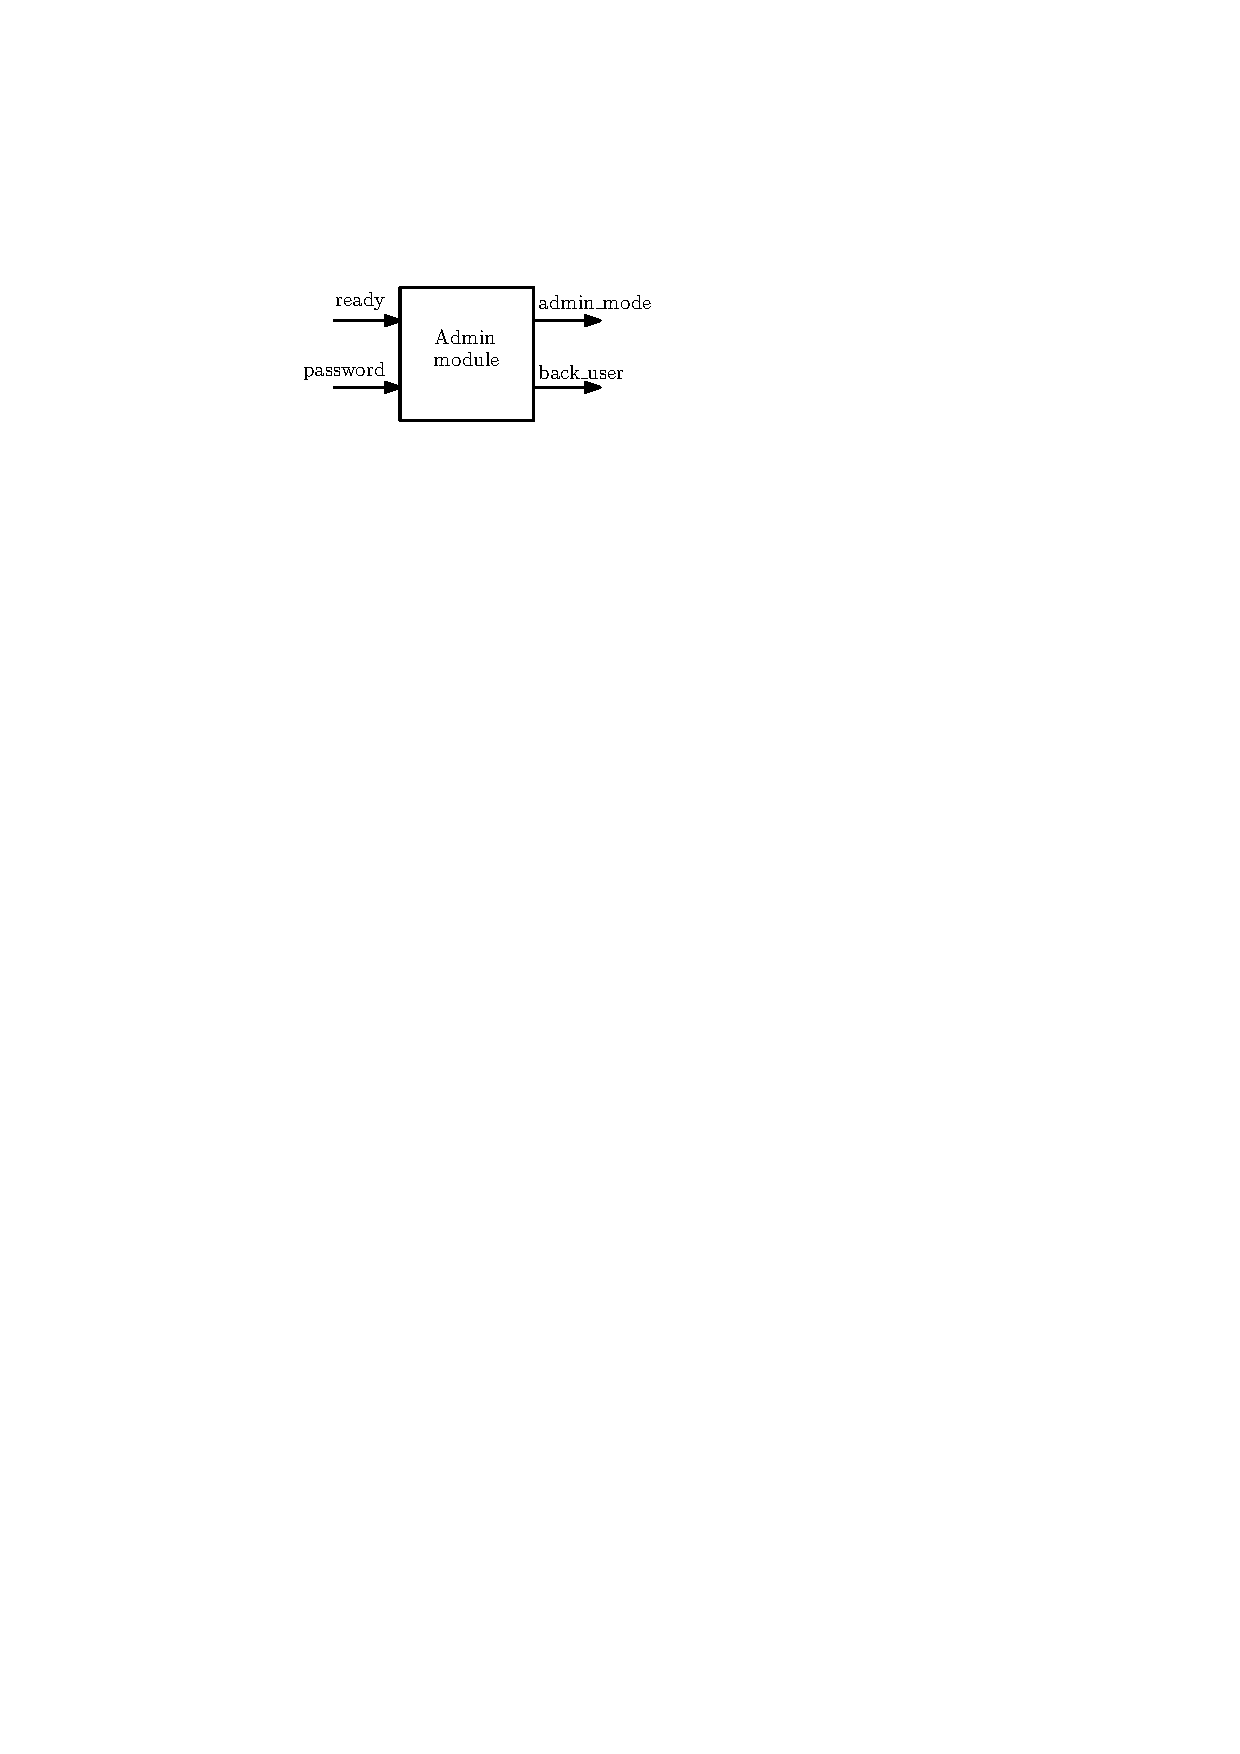
\includegraphics[width=0.5\textwidth]{images/admin.pdf}
	\caption{ماژول \texttt{user.v}}
	\label{ماژول user.v}
\end{figure}









\section*{{\titr بخش‌های اصلی }}
\addcontentsline{toc}{section}{{\fehrestContent بخش‌های اصلی}}


\subsection*{{\titr فاز صفر} (۱۰ + ۱۰) نمره} 
\addcontentsline{toc}{subsection}{{\fehrestContent فاز صفر}}

در این فاز شما باید مقدمات پروژه را حاضر کنید. این مقدمات شامل ابزارهای مورد استفاده در پروژه و همچنین طراحی \lr{FSM} های پروژه به‌صورت کلی است. مراحل این فاز عبارت اند از:

\begin{enumerate}
	\item
	\hyperref[subsubsec:github]{\textcolor{magenta}{راه اندازی مخزن \lr{GitHub}}}
	
	\item
	\hyperref[subsubsec:fsm]{\textcolor{magenta}{طراحی \lr{FSM} برای منطق پروژه}}
\end{enumerate}

در بخش بعد، هر یک از این موارد شرح داده شده اند.



\subsubsection*{{\titr راه‌اندازی مخزن GitHub} (۱۰) نمره}
\addcontentsline{toc}{subsubsection}{{\fehrestContent راه‌اندازی مخزن GitHub}}
\label{subsubsec:github}

همانطور که می‌دانید برای پروژه لازم است با گروهتان بر روی یک مخزن \lr{(repository)} گیت فعالیت کنید. برای ساختن این مخزن، کافیست وارد
\href{https://classroom.github.com/a/rBR982eM}{\textcolor{magenta}{\underline{این لینک}}} 
شوید.

ابتدا با لیستی مواجه می‌شوید که شماره دانشجویی تمام افراد در آن موجود است. شماره دانشجویی خود را بیابید و بر روی آن کلیک کنید.

\newpage
\Large \textbf{\\
}

در صفحه‌ی بعد شما باید تیم خود را انتخاب کنید. چنانچه نفر اول گروه خود (سازنده‌ی مخزن) هستید، باید یک تیم بسازید. تنها شماره‌ی گروه پروژه خود را در قسمت نام تیم وارد کنید و تیم را بسازید. نفرات بعدی گروه شما، باید تیم‌شان را از لیست تیم‌های موجود انتخاب کنند و نیازی به ایجاد تیم ندارند.

پس از این مراحل مخزن شما آماده خواهد شد و لینک آن در اختیارتان قرار خواهد گرفت. پس از آماده شدن این مخزن، هر یک از اعضای پروژه باید نام و شماره دانشجویی خود را به فایل \lr{README.md} اضافه کند.






\subsubsection*{{\titr طراحی FSM برای منطق پروژه} (۱۰) نمره}
\addcontentsline{toc}{subsubsection}{{\fehrestContent طراحی FSM برای منطق پروژه}}
\label{subsubsec:fsm}

همانطور که در بخش 
\hyperref[sec:detail]{\textcolor{magenta}{توضیحات کلی}}
مطرح شد، پروژه دارای ۳ ماژول اصلی است. در این قسمت از شما می‌خواهیم ۳ \lr{FSM} منطبق بر منطق ۳ ماژول \texttt{admin.v}، \texttt{user.v} و \texttt{main.v} رسم نمایید.

در این فاز نیازی به درنظر گرفتن جزئیات مسئله نمی‌باشد و صرفا طراحی کلیات این ۳ ماژول مفایت می‌کند.





\subsection*{{\titr فاز اول} (۸۰) نمره}
\addcontentsline{toc}{subsection}{{\fehrestContent فاز اول}}
پس از طراحی \lr{FSM} های کلی در فاز صفر و راه‌اندازی مخزن گیتهاب، در این فاز از پروژه نیاز است که جزئیات نیز درنظر گرفته شود و \lr{FSM} های طراحی شده تکمیل شود. پس از تکمیل \lr{FSM} ها نیاز است کدهای \lr{verilog} ماژول های توضیح داده شده در بخش 
\hyperref[sec:detail]{\textcolor{magenta}{توضیحات کلی}}
نوشته شود. 

تمامی ماژول ها باید قابل سنتز و پیاده سازی\footnote{\lr{Implementation}} باشند چرا که می‌بایست به صورت عملی بر روی بُرد پروگرام شده و تست شود.

اکیدا توصیه می‌شود مرحله به مرحله کد‌ها را نوشته و برای هر ماژول \lr{Testbench} بنویسید و از صحت عملکرد ماژول مطمئن شوید، اما اجباری به نوشتن \lr{Testbench} نیست.



\newpage
\Large \textbf{\\
}



\section*{{\titr بخش‌های امتیازی} (۲۰ + ۲۵) نمره}
\addcontentsline{toc}{section}{{\fehrestContent بخش‌های امتیازی}}

از این قسمت به بعد وارد بخش‌های امتیازی پروژه می شویم. دقت کنید که این بخش های هم بسیار آموزنده و کاربردی هستند و هم می تواند به نمره پروژه شما به اندازه قابل توجهی اضافه کند. :)


\subsection*{{\titr وضعیت دریافت ورودی} (۲۰) نمره}
\addcontentsline{toc}{subsection}{{\fehrestContent وضعیت دریافت ورودی}}
در حالت اجباری و غیر امتیازی پروژه، تمامی ورودی ها با استفاده از \lr{Dip switch} ها و \lr{Push button} ها داده می‌شد. در این بخش می‌توانید به صورتی طراحی را تغییر دهید که سیستم شما ورودی‌ها را با استفاده از صفحه کلید\footnote{\lr{Keypad}} دریافت کند.

بُرد های آزمایشگاه مجهز به صفحه کلید نمی‌باشند اما می‌توانید آن را به‌صورت مجزا از مسئول آزمایشگاه تهیه کرده و ماژولی به‌نام \texttt{keypad.v} نوشته و آن را به بُرد متصل کنید. نمونه ای از صفحه‌کلید های رایج در ادامه آورده شده است.


\begin{figure}[h]
	\centering
	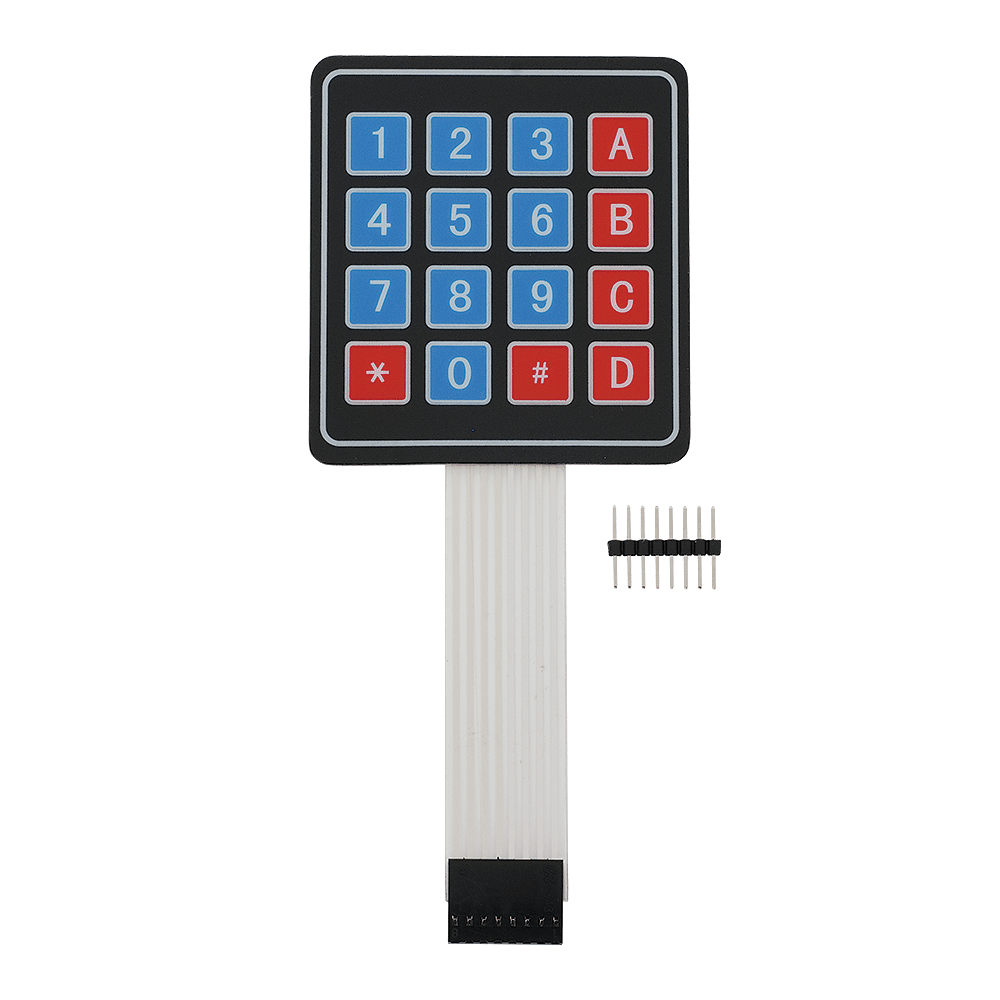
\includegraphics[width=0.4\textwidth]{images/keypad.png}
	\caption{صفحه کلید}
	\label{صفحه کلید}
\end{figure}




\newpage
\Large \textbf{\\
}




\subsection*{{\titr وضعیت نمایش} (۲۵) نمره}
\addcontentsline{toc}{subsection}{{\fehrestContent وضعیت دریافت ورودی}}
در این قسمت می‌توانید برای نمایش وضعیت موجودی اجناس، قیمت‌ها، شماره کاربر و مانده حساب از \lr{LCD} کاراکتری استفاده نمایید. بُرد های آزمایشگاه مجهز به \lr{LCD} کاراکتری هستند. 

برای انجام این قسمت می‌بایست ماژولی به نام \texttt{lcd.v} بنویسید. در ادامه نمونه‌ای از \texttt{LCD} های رایج آورده شده است.


\begin{figure}[h]
	\centering
	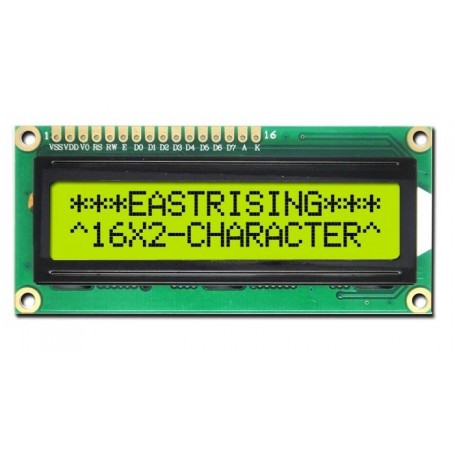
\includegraphics[width=0.5\textwidth]{images/lcd.jpg}
	\caption{\lr{LCD} کاراکتری}
	\label{LCD کاراکتری}
\end{figure}



\end{document}